\appendix

\chapter{Anhang I}
\label{ch:appendix_1}

\section{Literaturrecherche}
\label{sec:appendix_search_filter}

\begin{table}
    \centering
    \begin{tabular}{l}
        \hline
        test \\
        \toprule
        test 2 \\
        \toprule
    \end{tabular}
    \caption{Filter}
\end{table}

\begin{figure}[htb]
    \centering
    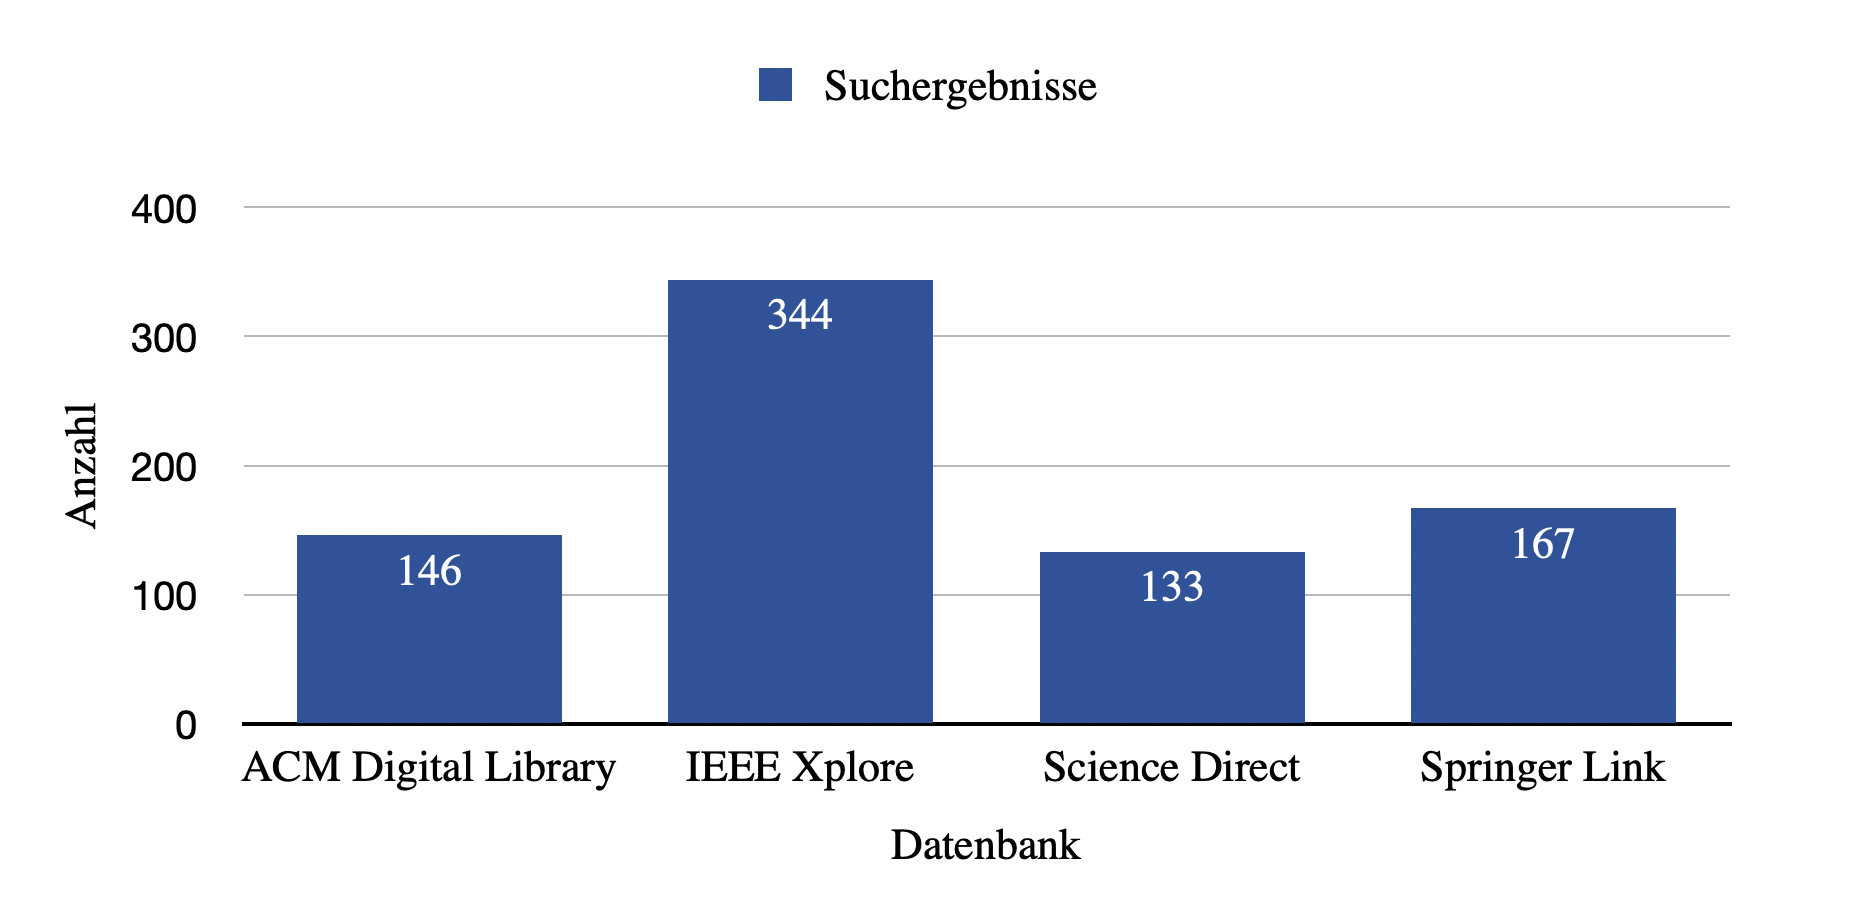
\includegraphics[width=0.75\linewidth]{contents/04_literature_review/res/database_results.png}
    \caption{Anzahl der Suchergebnisse pro Datenbank}
\end{figure}

\begin{table}
    \begin{center}
        \begin{tabular}{p{.3\textwidth}p{.64\textwidth}}
            \hline
            Kontext                   & Quellen \\
            \toprule
            Allgemein                           &
                \cite{chazette_end-users_nodate} \cite{chazette2020explainability} \cite{chazette_knowledge_nodate} \cite{eiband_impact_2019} \cite{kohl_explainability_2019} \cite{ribera2019can} \cite{lim_2009_assessing} \\
            \tablerowspacing
            Intelligente Systeme (z.B. XAI)      & 
                \cite{waa_evaluating_2021} \cite{mucha_interfaces_2021} \cite{sokol_explainability_2020}  \cite{abdulrahman_belief-based_2019} \cite{brennen_what_2020} \cite{schaffer_i_2019} \cite{weitz_you_2019} \cite{riveiro_thats_2021} \cite{martin_developing_2019} \cite{martin_evaluating_2021} \cite{rosenfeld_explainability_2019} \cite{cassens_ambient_2019} \cite{cirqueira_scenario-based_2020}  \cite{ehsan_human-centered_2020} \cite{rjoob_towards_2021} \cite{thomson_knowledge--information_2020} \cite{chari_explanation_2020} \cite{sokol_one_2020}  \cite{neerincx_using_2018} \cite{schrills_color_2020} \cite{sovrano_modelling_2020} \cite{gunning2019darpa} \cite{doshi2017towards} \cite{cheng2019explaining}\\
            \tablerowspacing
            Empfehlungssysteme                  & 
                \cite{tintarev_designing_nodate} \cite{sato_context_nodate} \cite{balog_measuring_2020}  \cite{kouki_user_2017} \cite{tsai_evaluating_2019} \cite{hernandez-bocanegra_effects_2020} \cite{kunkel_let_2019} \cite{tintarev2015explaining} \cite{sato_action-triggering_2019} \cite{tsai_effects_2020} \cite{nunes_systematic_2017} \cite{tintarev2007survey}
            \\
            \tablerowspacing
            Autonomes Fahren                    &
                \cite{wiegand_id_2020} \cite{haspiel_explanations_2018} \cite{koo_understanding_2016} \cite{koo_why_2015} \cite{wiegand2019drive} \cite{du2019look}
            \\
            \tablerowspacing
            Mensch-Roboter-Interaktion          &
                \cite{stange_effects_2021} \cite{kaptein_personalised_2017} \cite{zolotas_towards_2019} \cite{wang_is_2018} \cite{zhu_effects_2020}
            \\
            \tablerowspacing
            Spezifische Domänen                 &
                \cite{yamada_evaluating_2016} \cite{zahedi_towards_2019}
            \\
            \toprule
        \end{tabular}
    \end{center}
    \caption{Kontext innerhalb von Erklärbaren Systemen, der von den Arbeiten untersucht wurde}
\end{table}


\section{Workshop}

\section{Workshop-Protokoll: Integration von Erklärungen in NUNAV}
\label{sec:appendix_workshop_protocol}

\section{Studienergebnisse}
\label{sec:appendix_study_results}

\begin{table}
    \begin{center}
        \begin{tabular}{|c|c|c|c|c|}
            \hline
            & \textbf{Gruppe 1} & \textbf{Gruppe 2} & \textbf{Gruppe 3} & \textbf{Gruppe 4} \\ \hline
            \textbf{Gruppe 1}   & 1.000000 & 1.000000 & 0.219884 & 0.008222 \\ \hline
            \textbf{Gruppe 2}   & 1.000000 & 1.000000 & 0.860586 & 0.000912 \\ \hline
            \textbf{Gruppe 3}   & 0.219884 & 0.860586 & 1.000000 & 0.000005 \\ \hline
            \textbf{Gruppe 4}   & 0.008222 & 0.000912 & 0.000005 & 1.000000 \\ \hline
        \end{tabular}
    \end{center}
    
    \caption{Signifikanzniveau $ p $ im paarweisen Vergleich der Anzahl der Routenabweichungen pro Kilometer zwischen den Studiengruppen }
    \label{tab:study_offroute_significance_results}
\end{table}

\section{Helcenter Collaborative Routing}
\label{sec:help_center_collaboratrive_routing}


\section{Helcenter Routeneinflüsse}
\label{sec:help_center_routing_data}


\section{vollständige Screenshots zum Verkehrsaufkommen}
\label{sec:appendix_traffic_volume}

\begin{figure}[htb!]
    \centering
    \subfloat[1. Prototyp zur Positionierung der \textit{Affordance}]
    {
        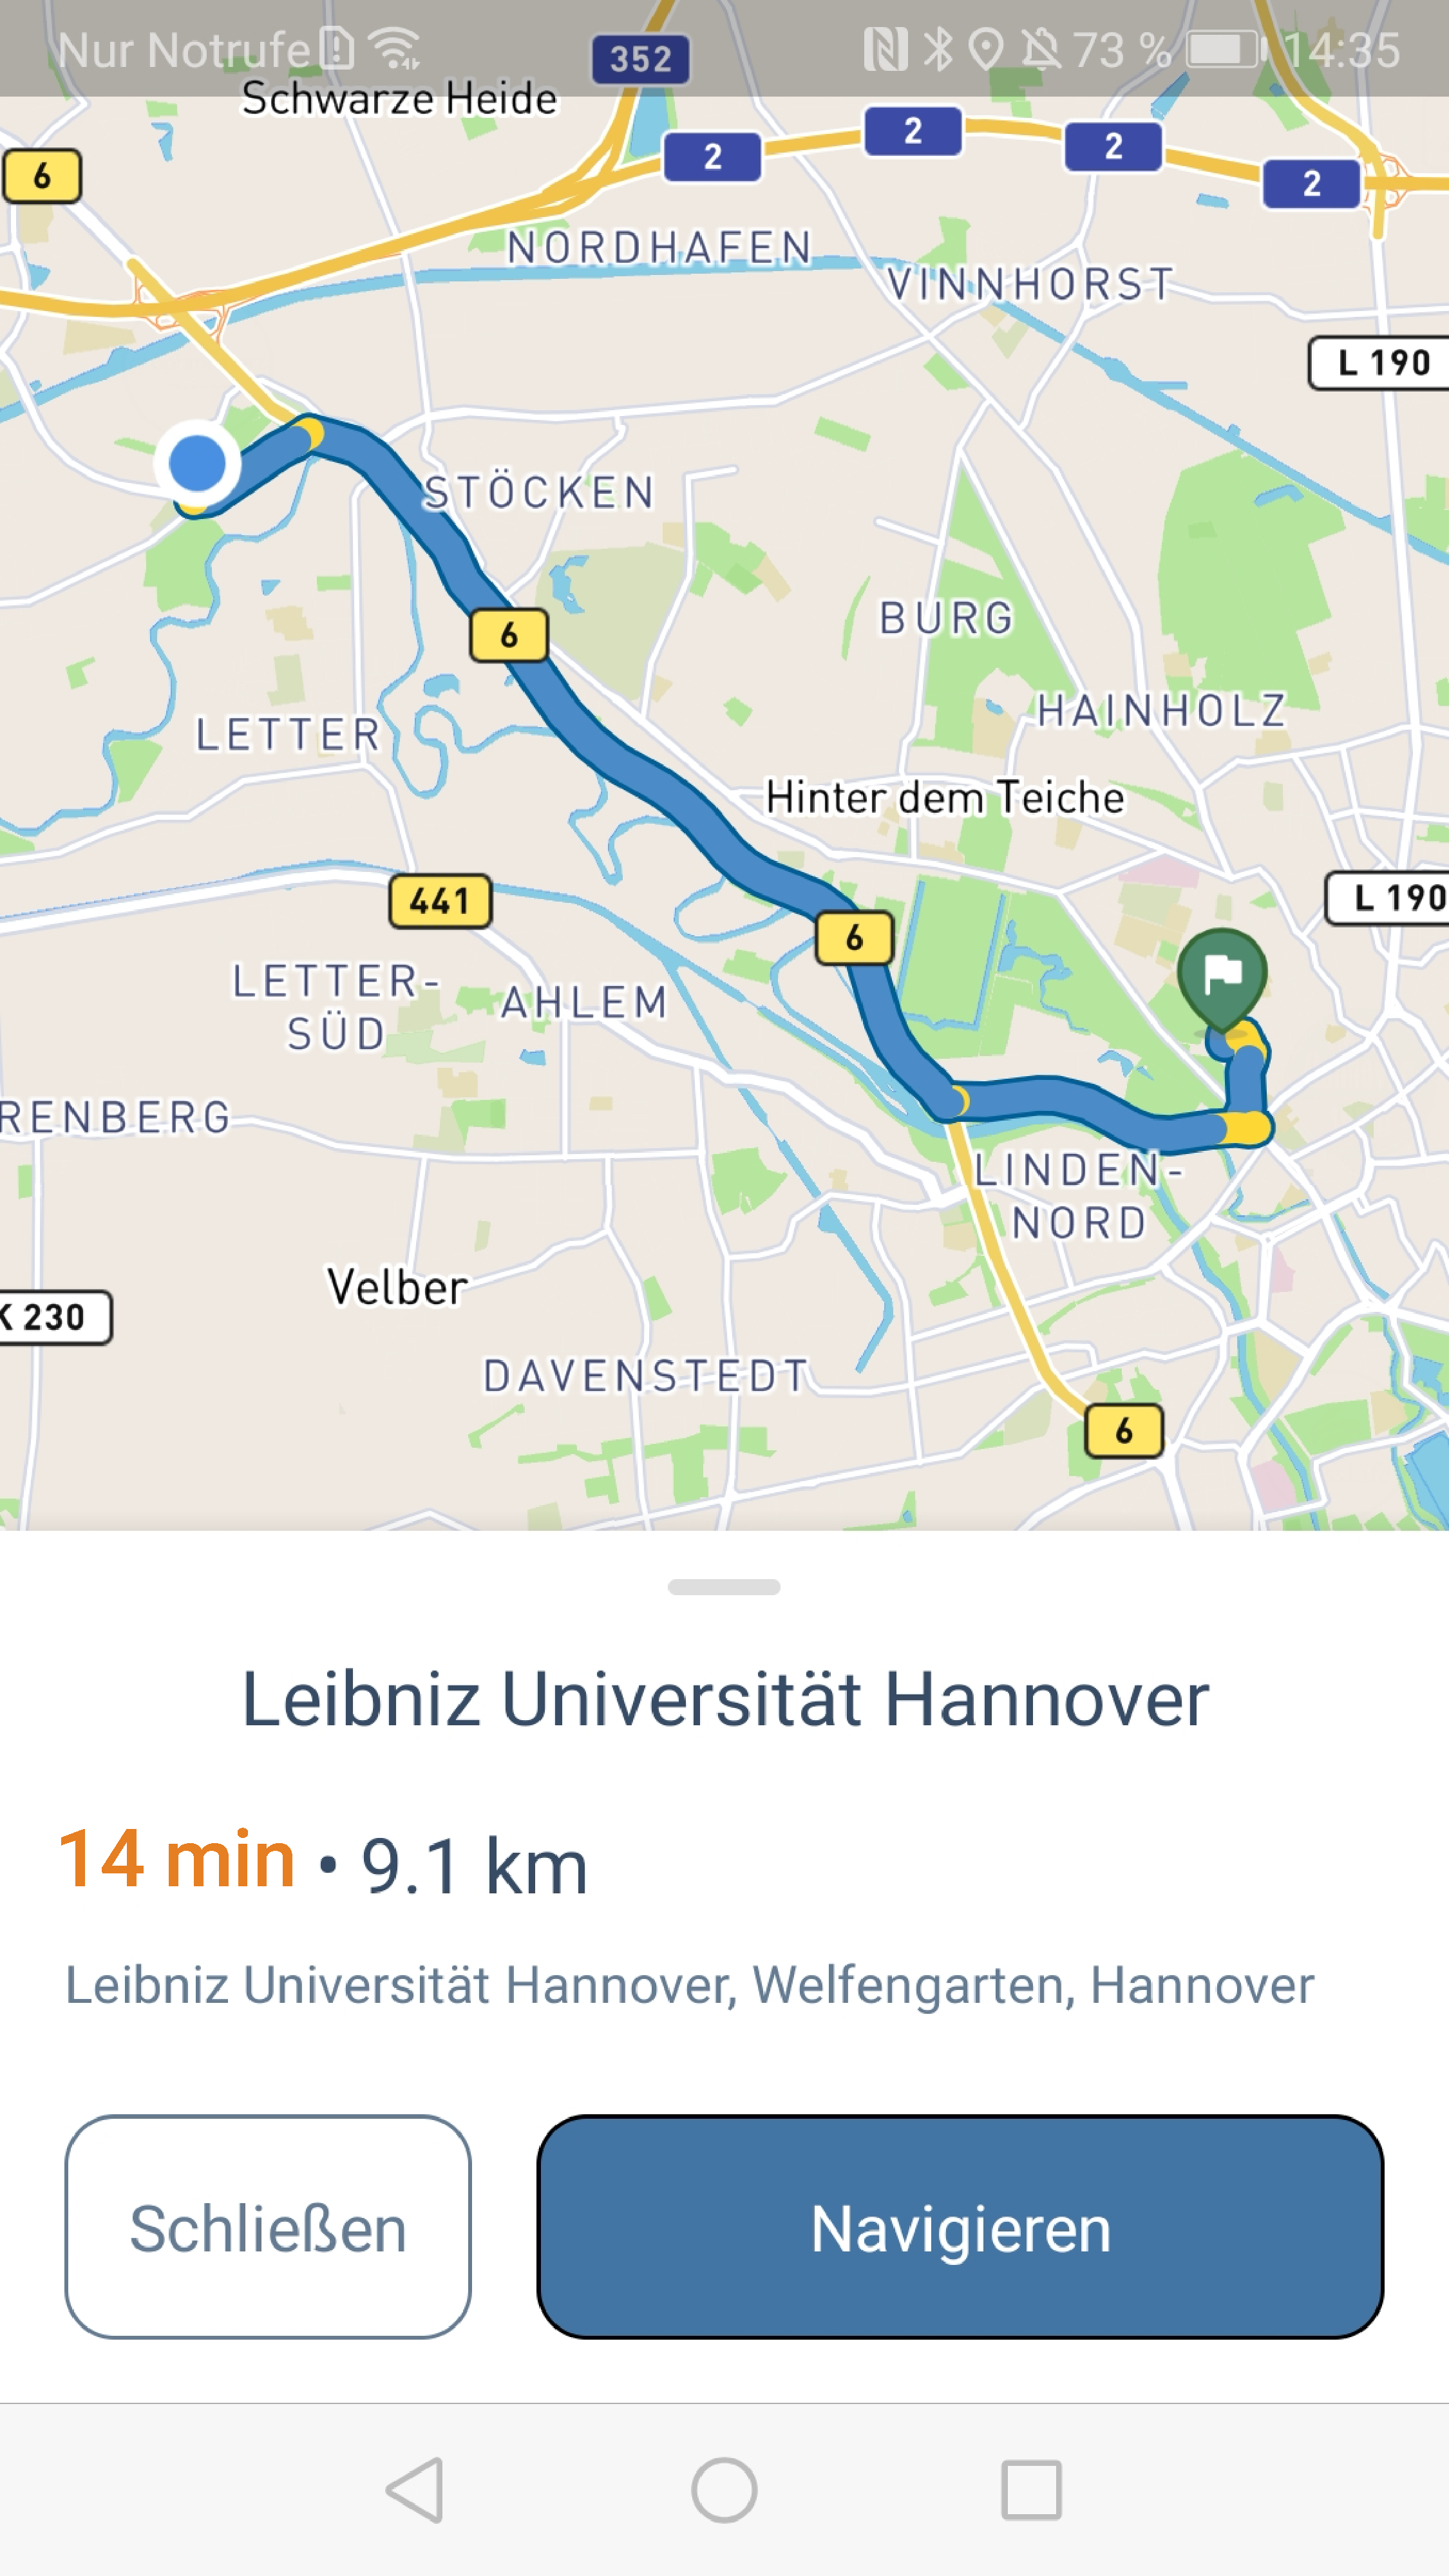
\includegraphics[width=.27\linewidth]{contents/06_model_evaluation/01_integration/res/03_traffic_volume/prototype_11.pdf}
    }
    \hspace{.055\linewidth}
    \subfloat[Alternativer Prototyp zur Positionierung der \textit{Affordance}]
    {
        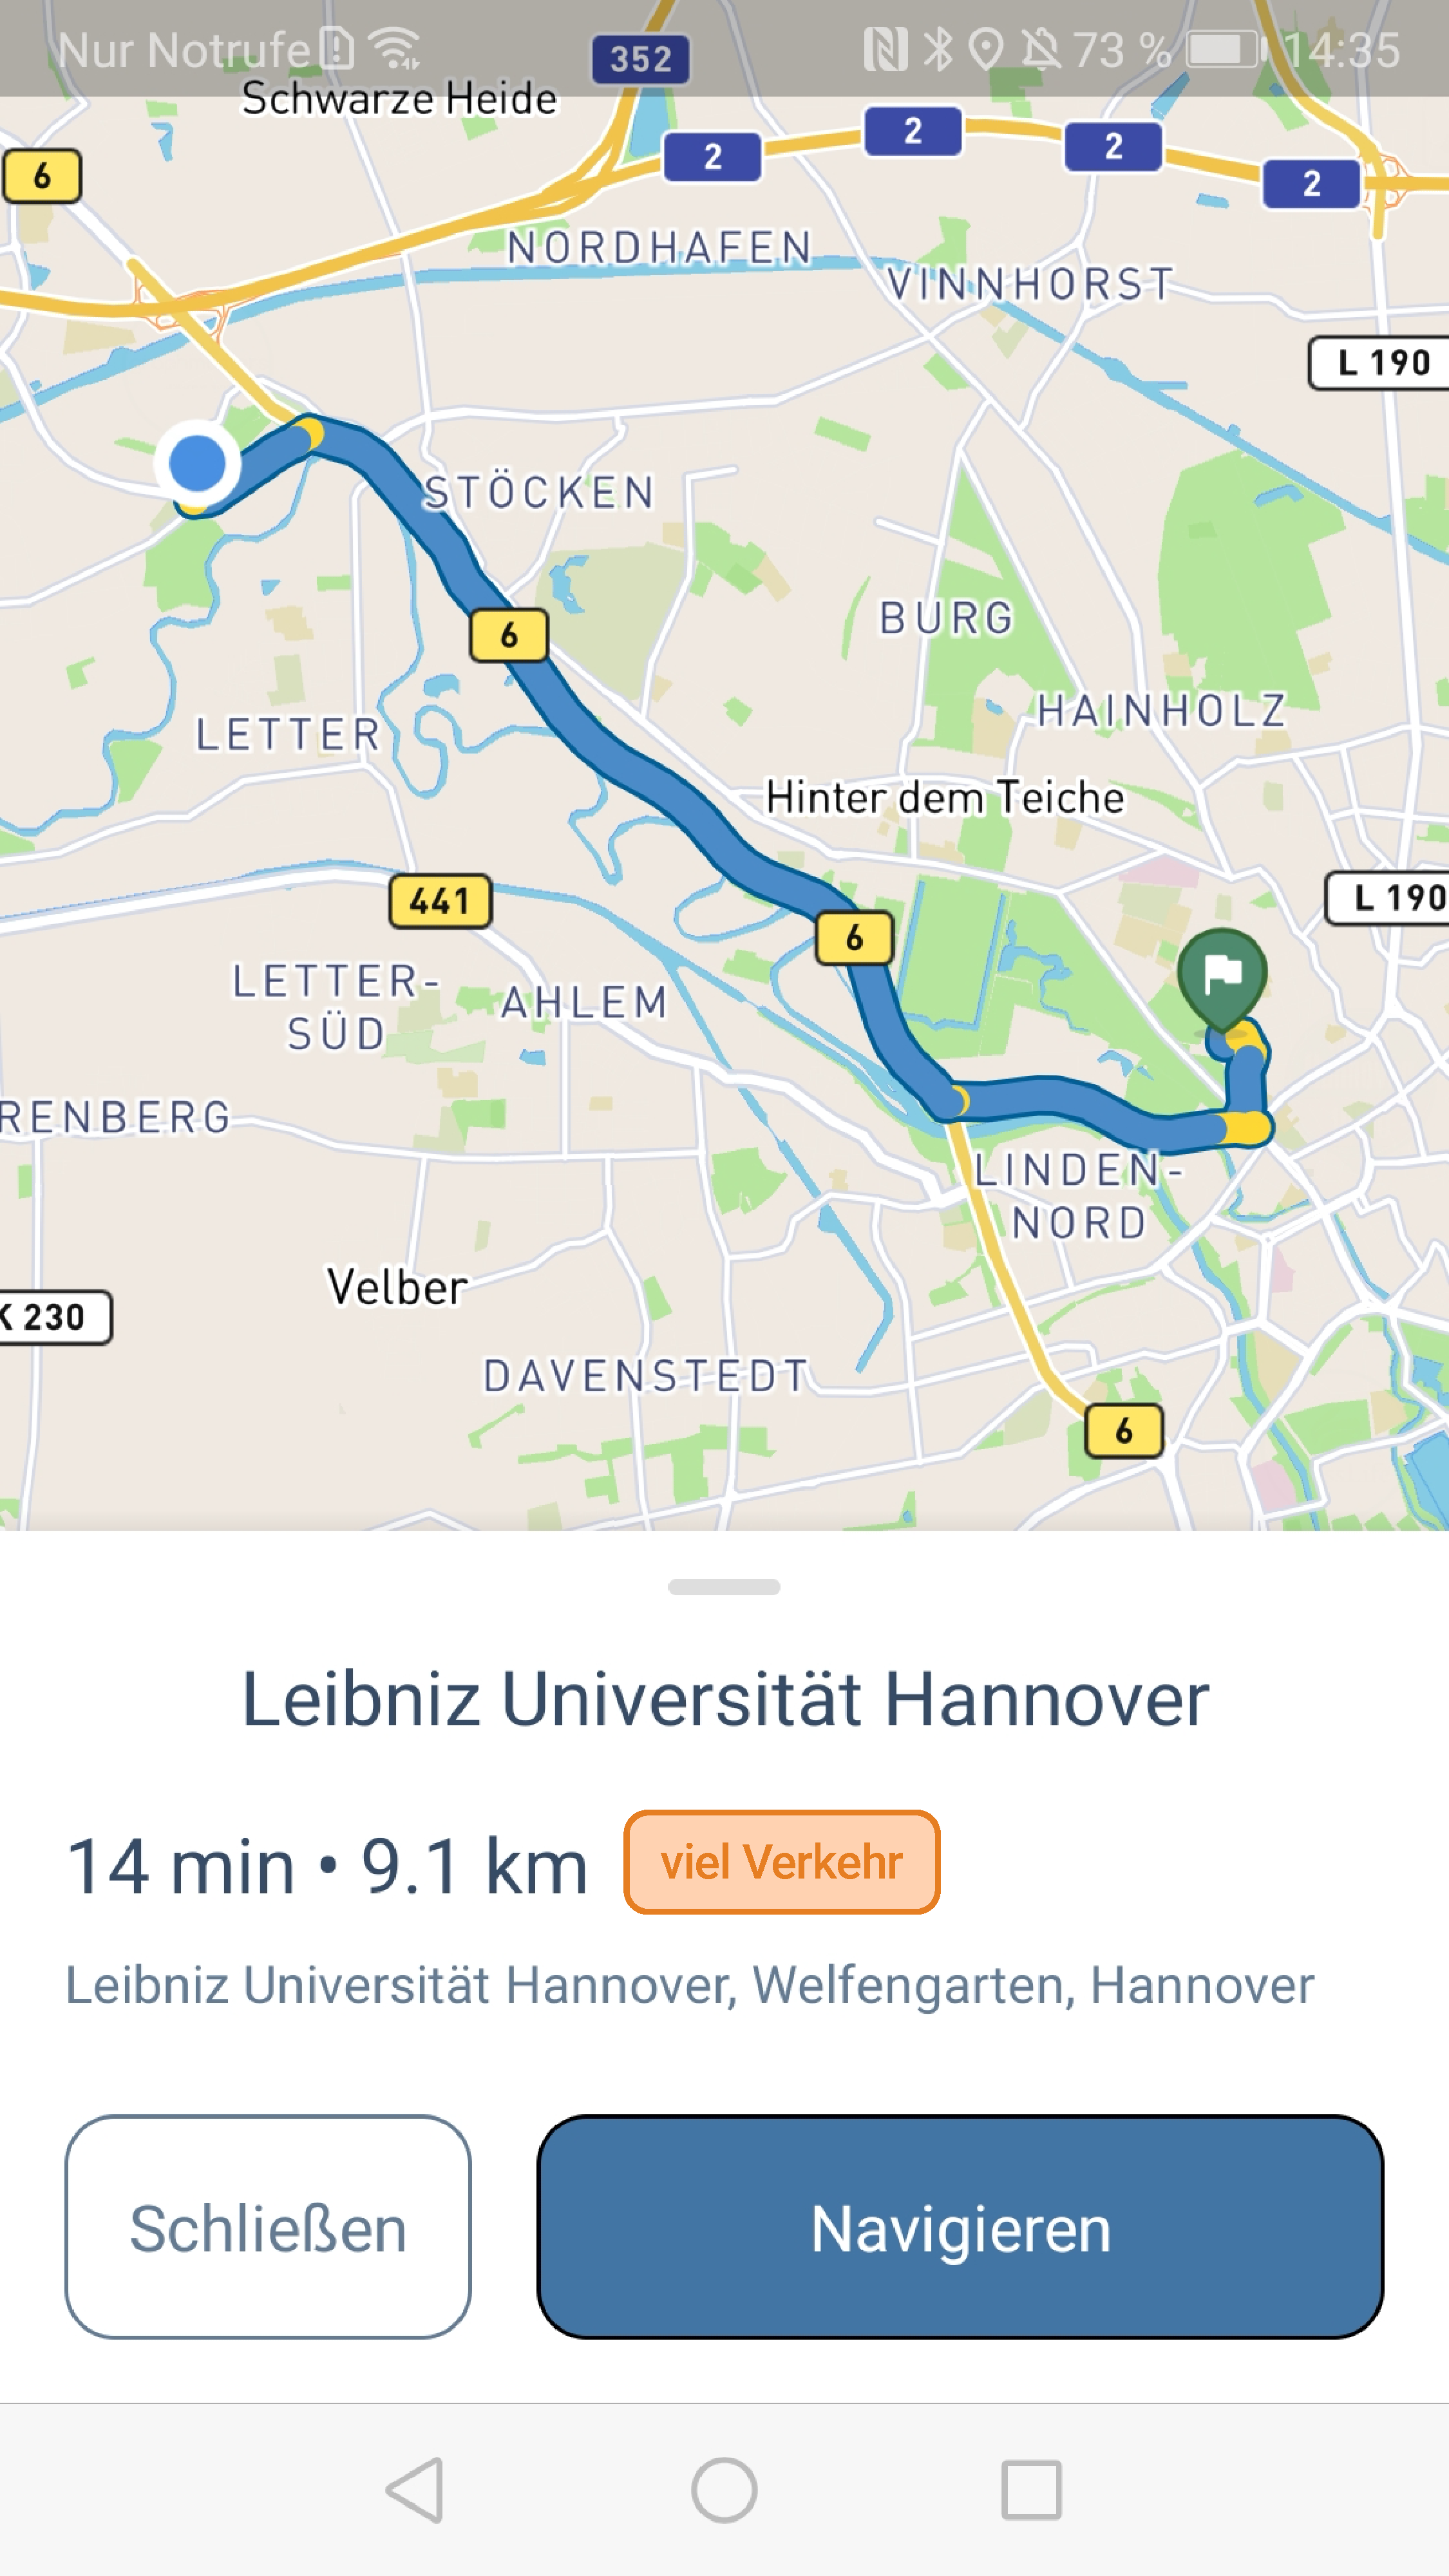
\includegraphics[width=.27\linewidth]{contents/06_model_evaluation/01_integration/res/03_traffic_volume/prototype_12.pdf}
    }
    \hspace{.055\linewidth}
    \subfloat[Finales Design der kurzen Erklärung]
    {
        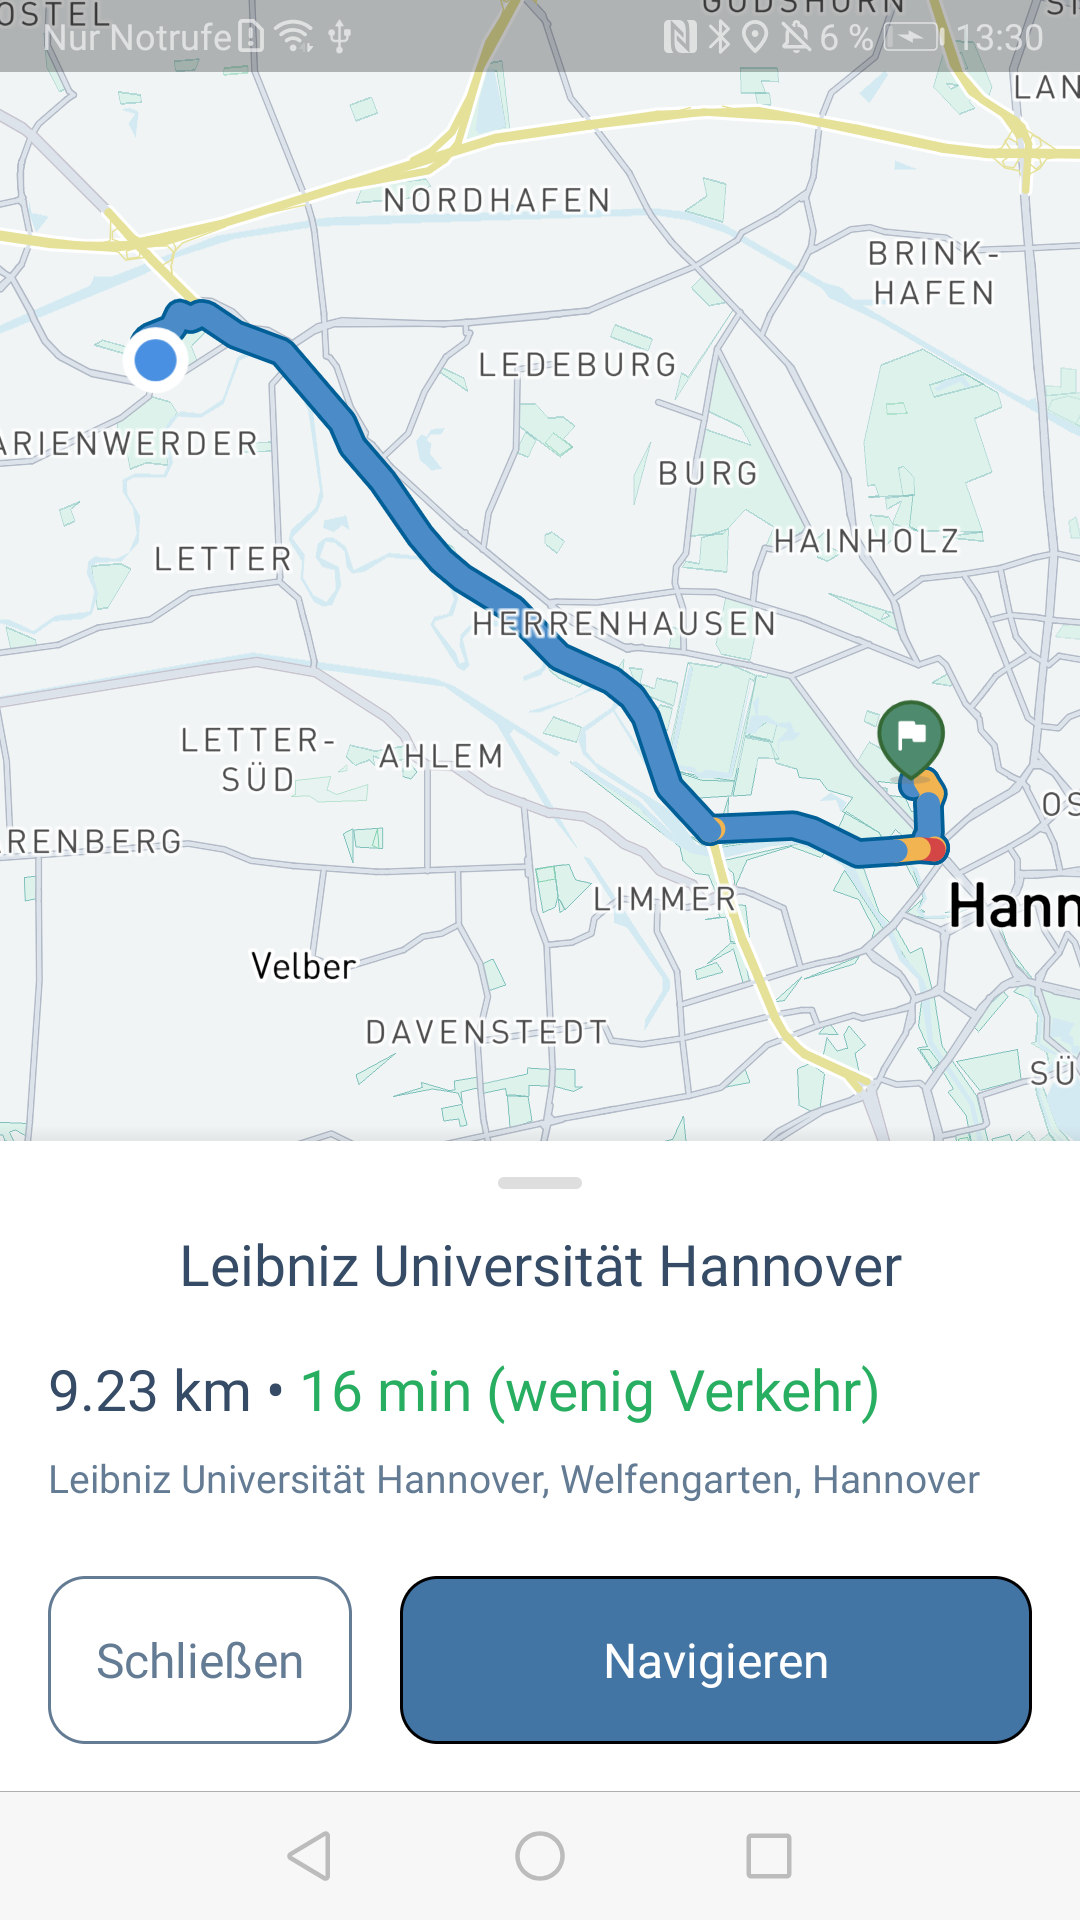
\includegraphics[width=.27\linewidth]{contents/06_model_evaluation/01_integration/res/03_traffic_volume/final_10.png}
    }
    \caption{Prototyp und finale Designs für die Erklärung zum kollaborativem Routing}
\end{figure}

\begin{figure}[htb!]
    \centering
    \subfloat[1. Prototyp zur Positionierung der \textit{Affordance}]
    {
        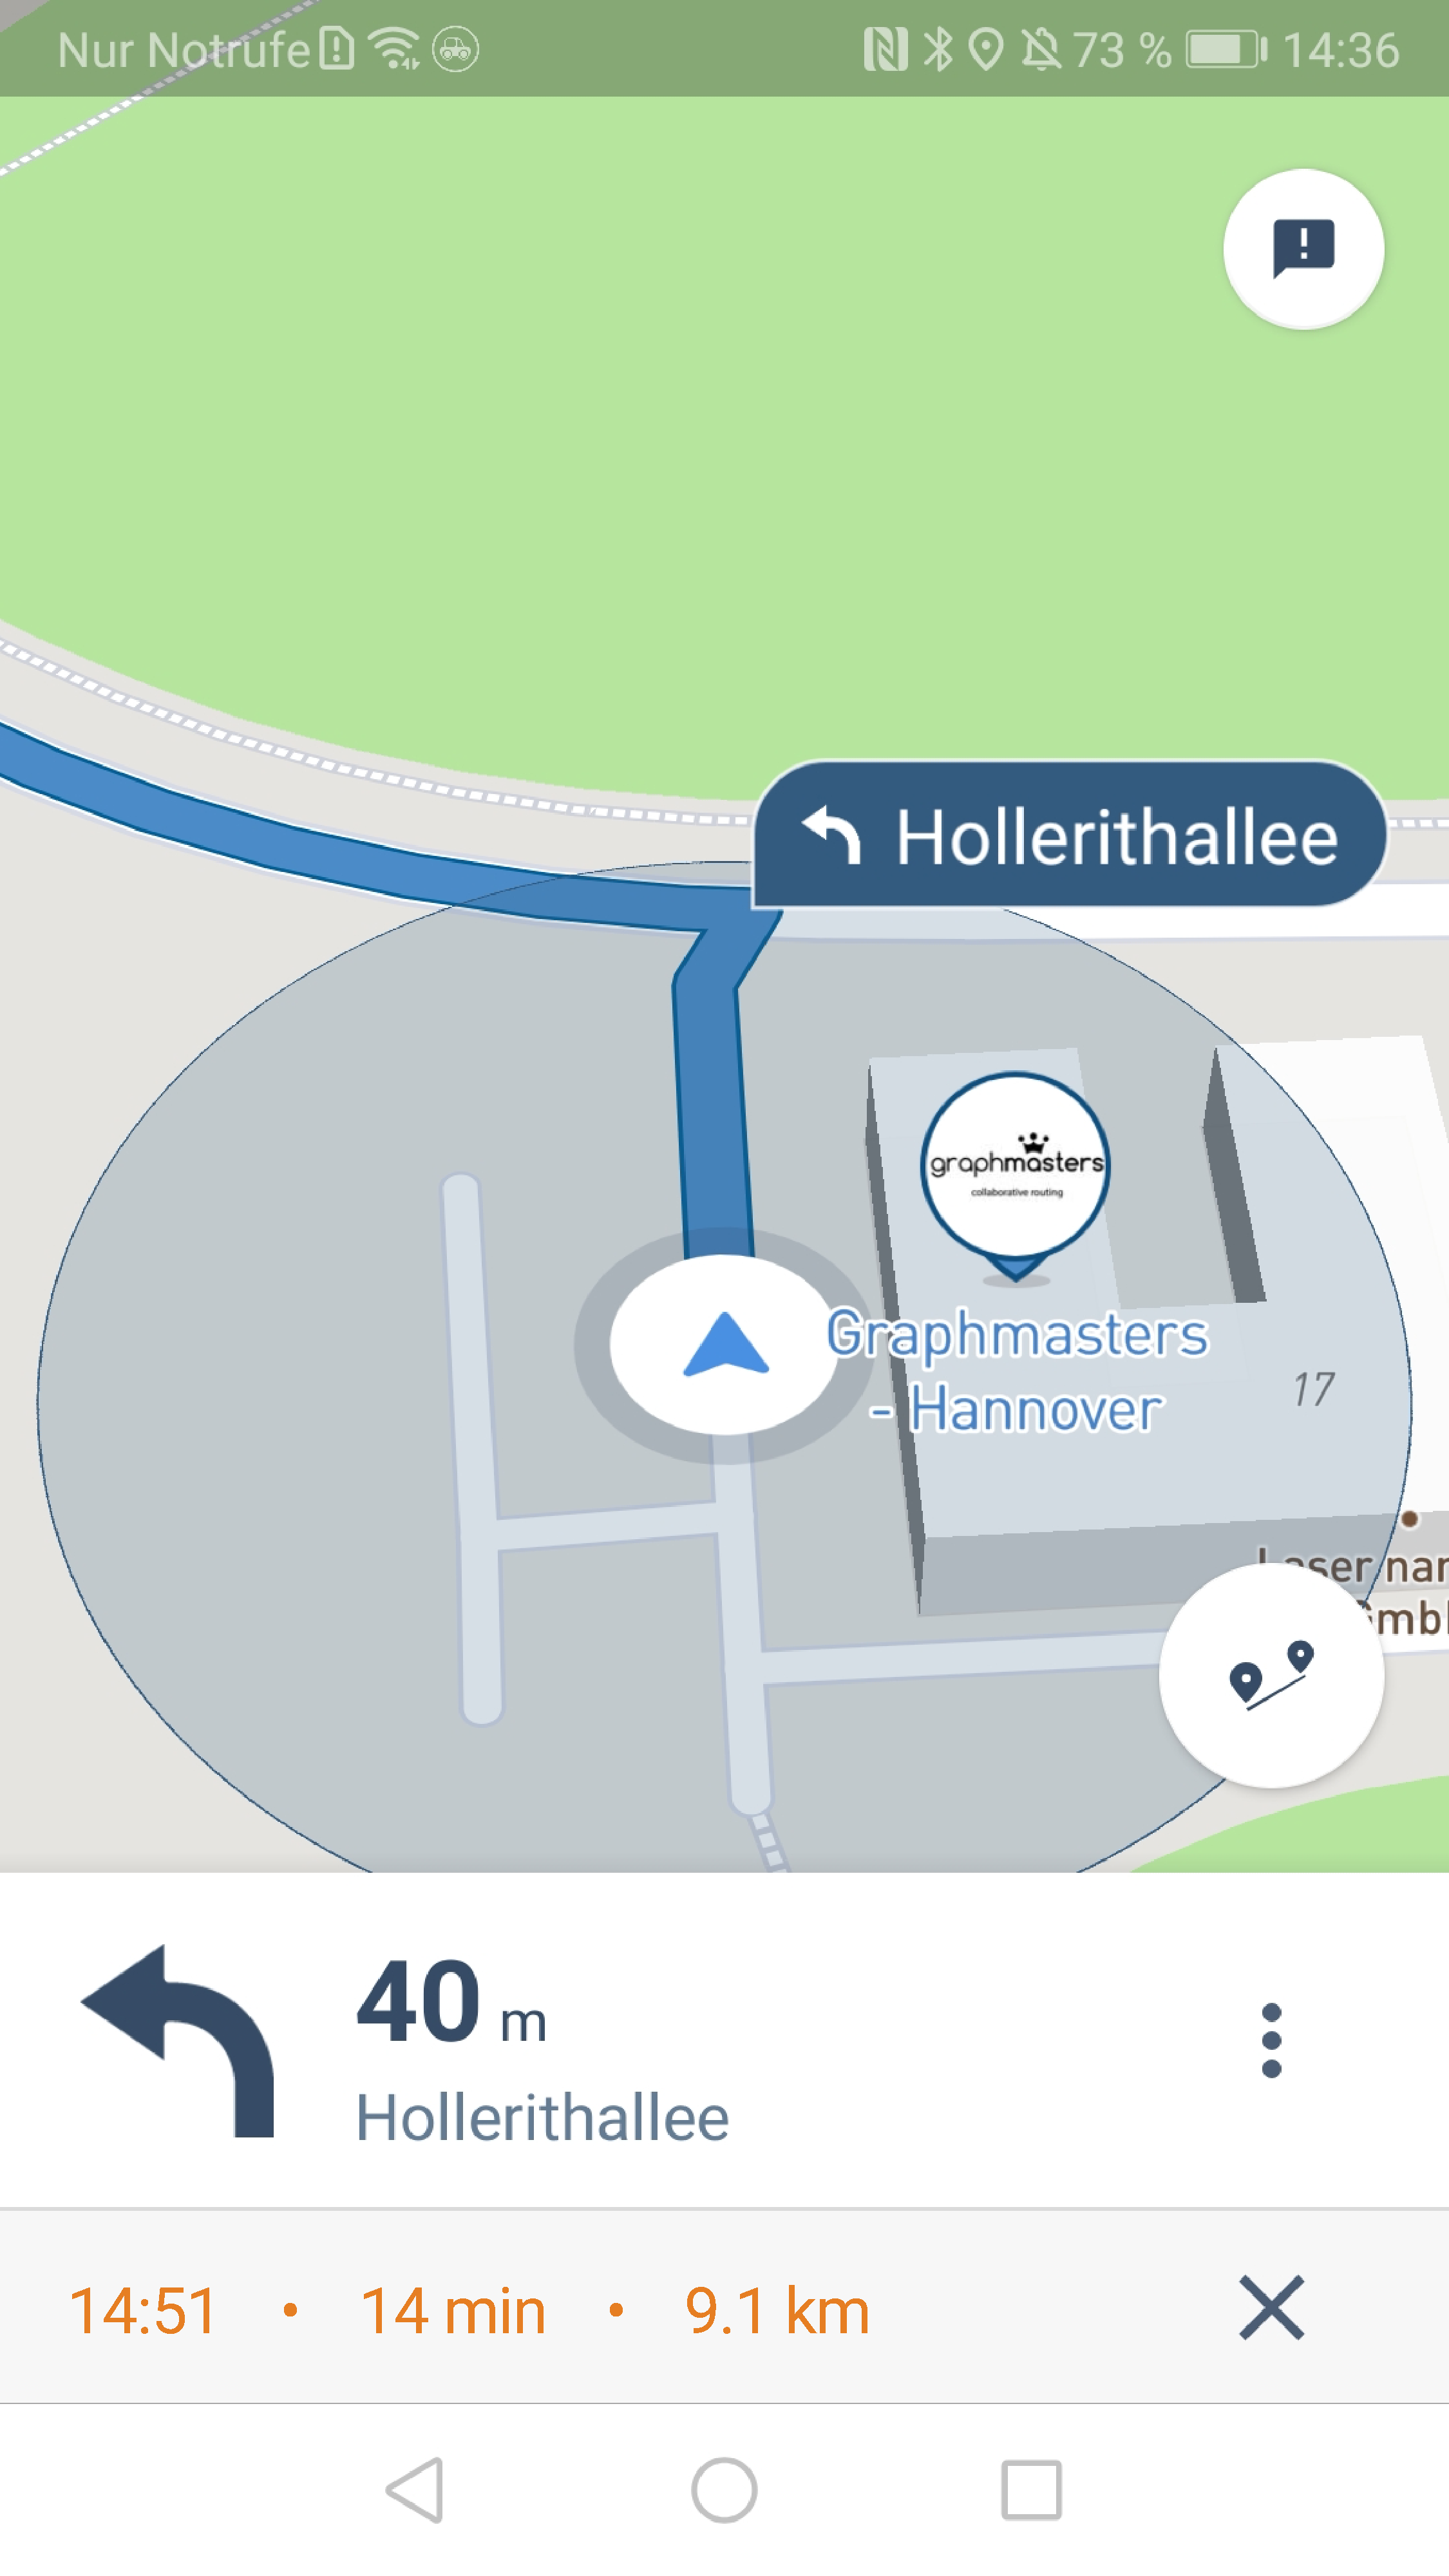
\includegraphics[width=.27\linewidth]{contents/06_model_evaluation/01_integration/res/03_traffic_volume/prototype_21.pdf}
    }
    \hspace{.055\linewidth}
    \subfloat[Alternativer Prototyp zur Positionierung der \textit{Affordance}]
    {
        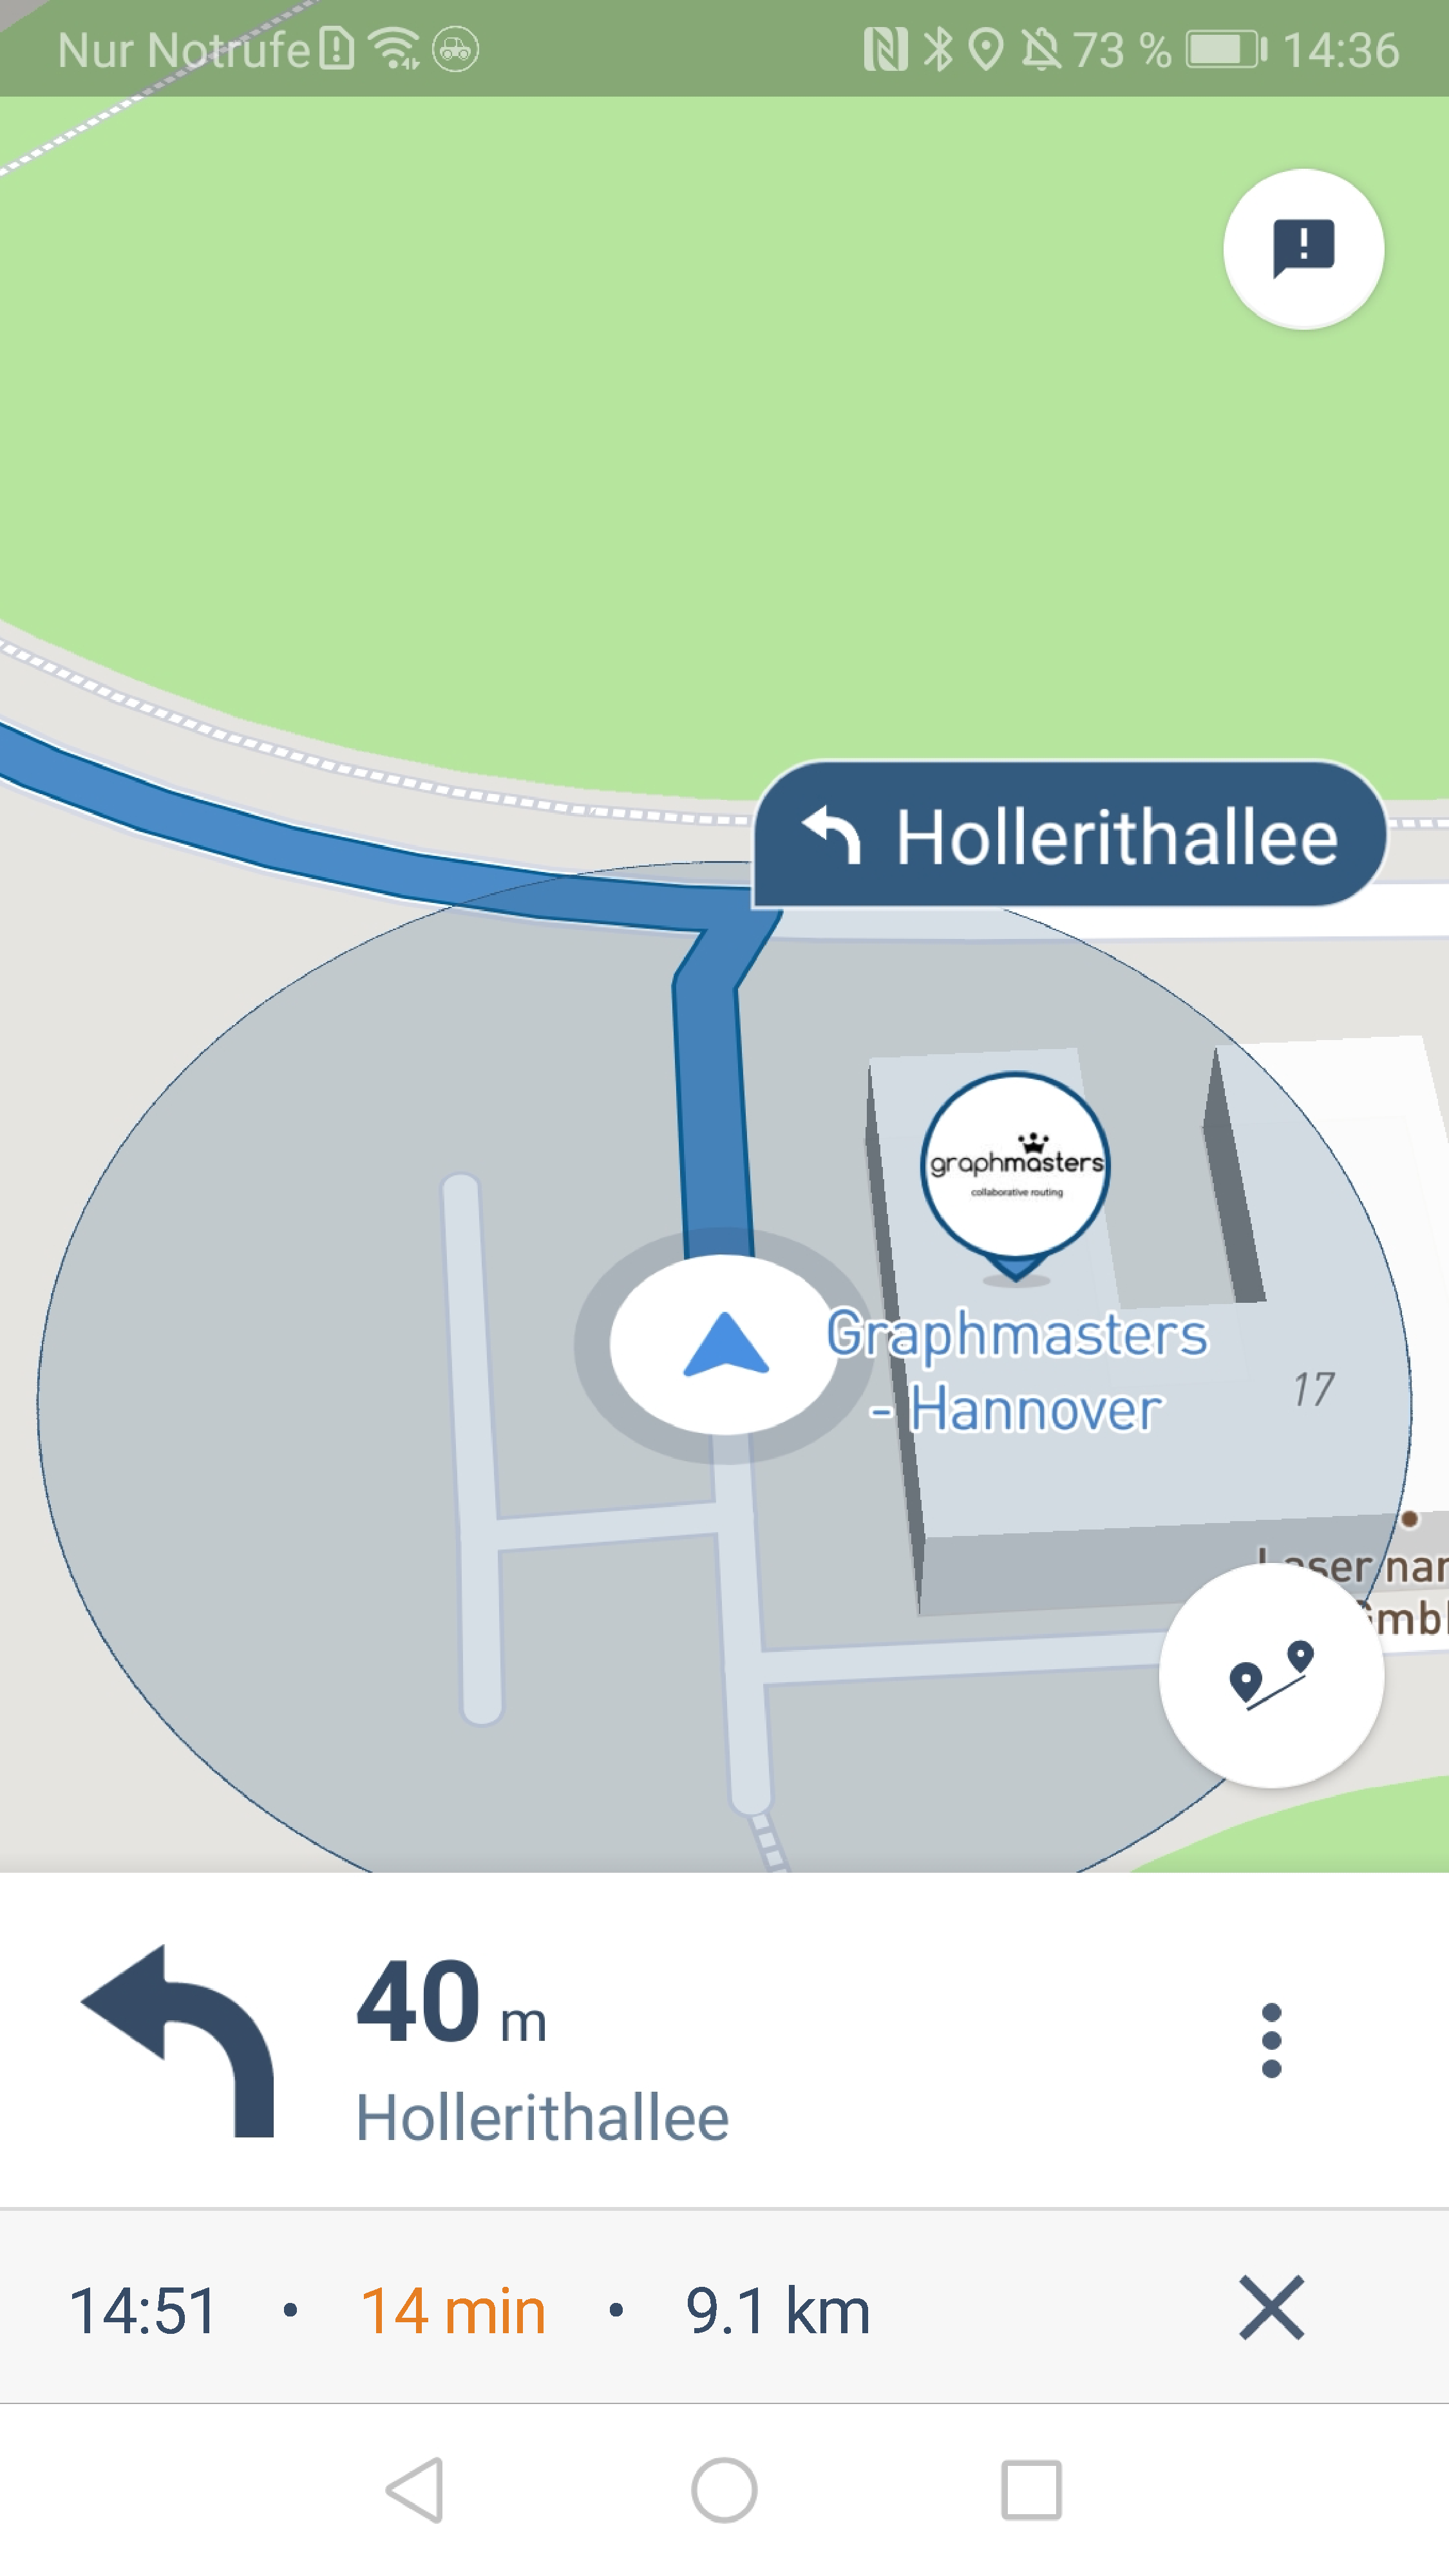
\includegraphics[width=.27\linewidth]{contents/06_model_evaluation/01_integration/res/03_traffic_volume/prototype_22.pdf}
    }
    \hspace{.055\linewidth}
    \subfloat[Finales Design der kurzen Erklärung]
    {
        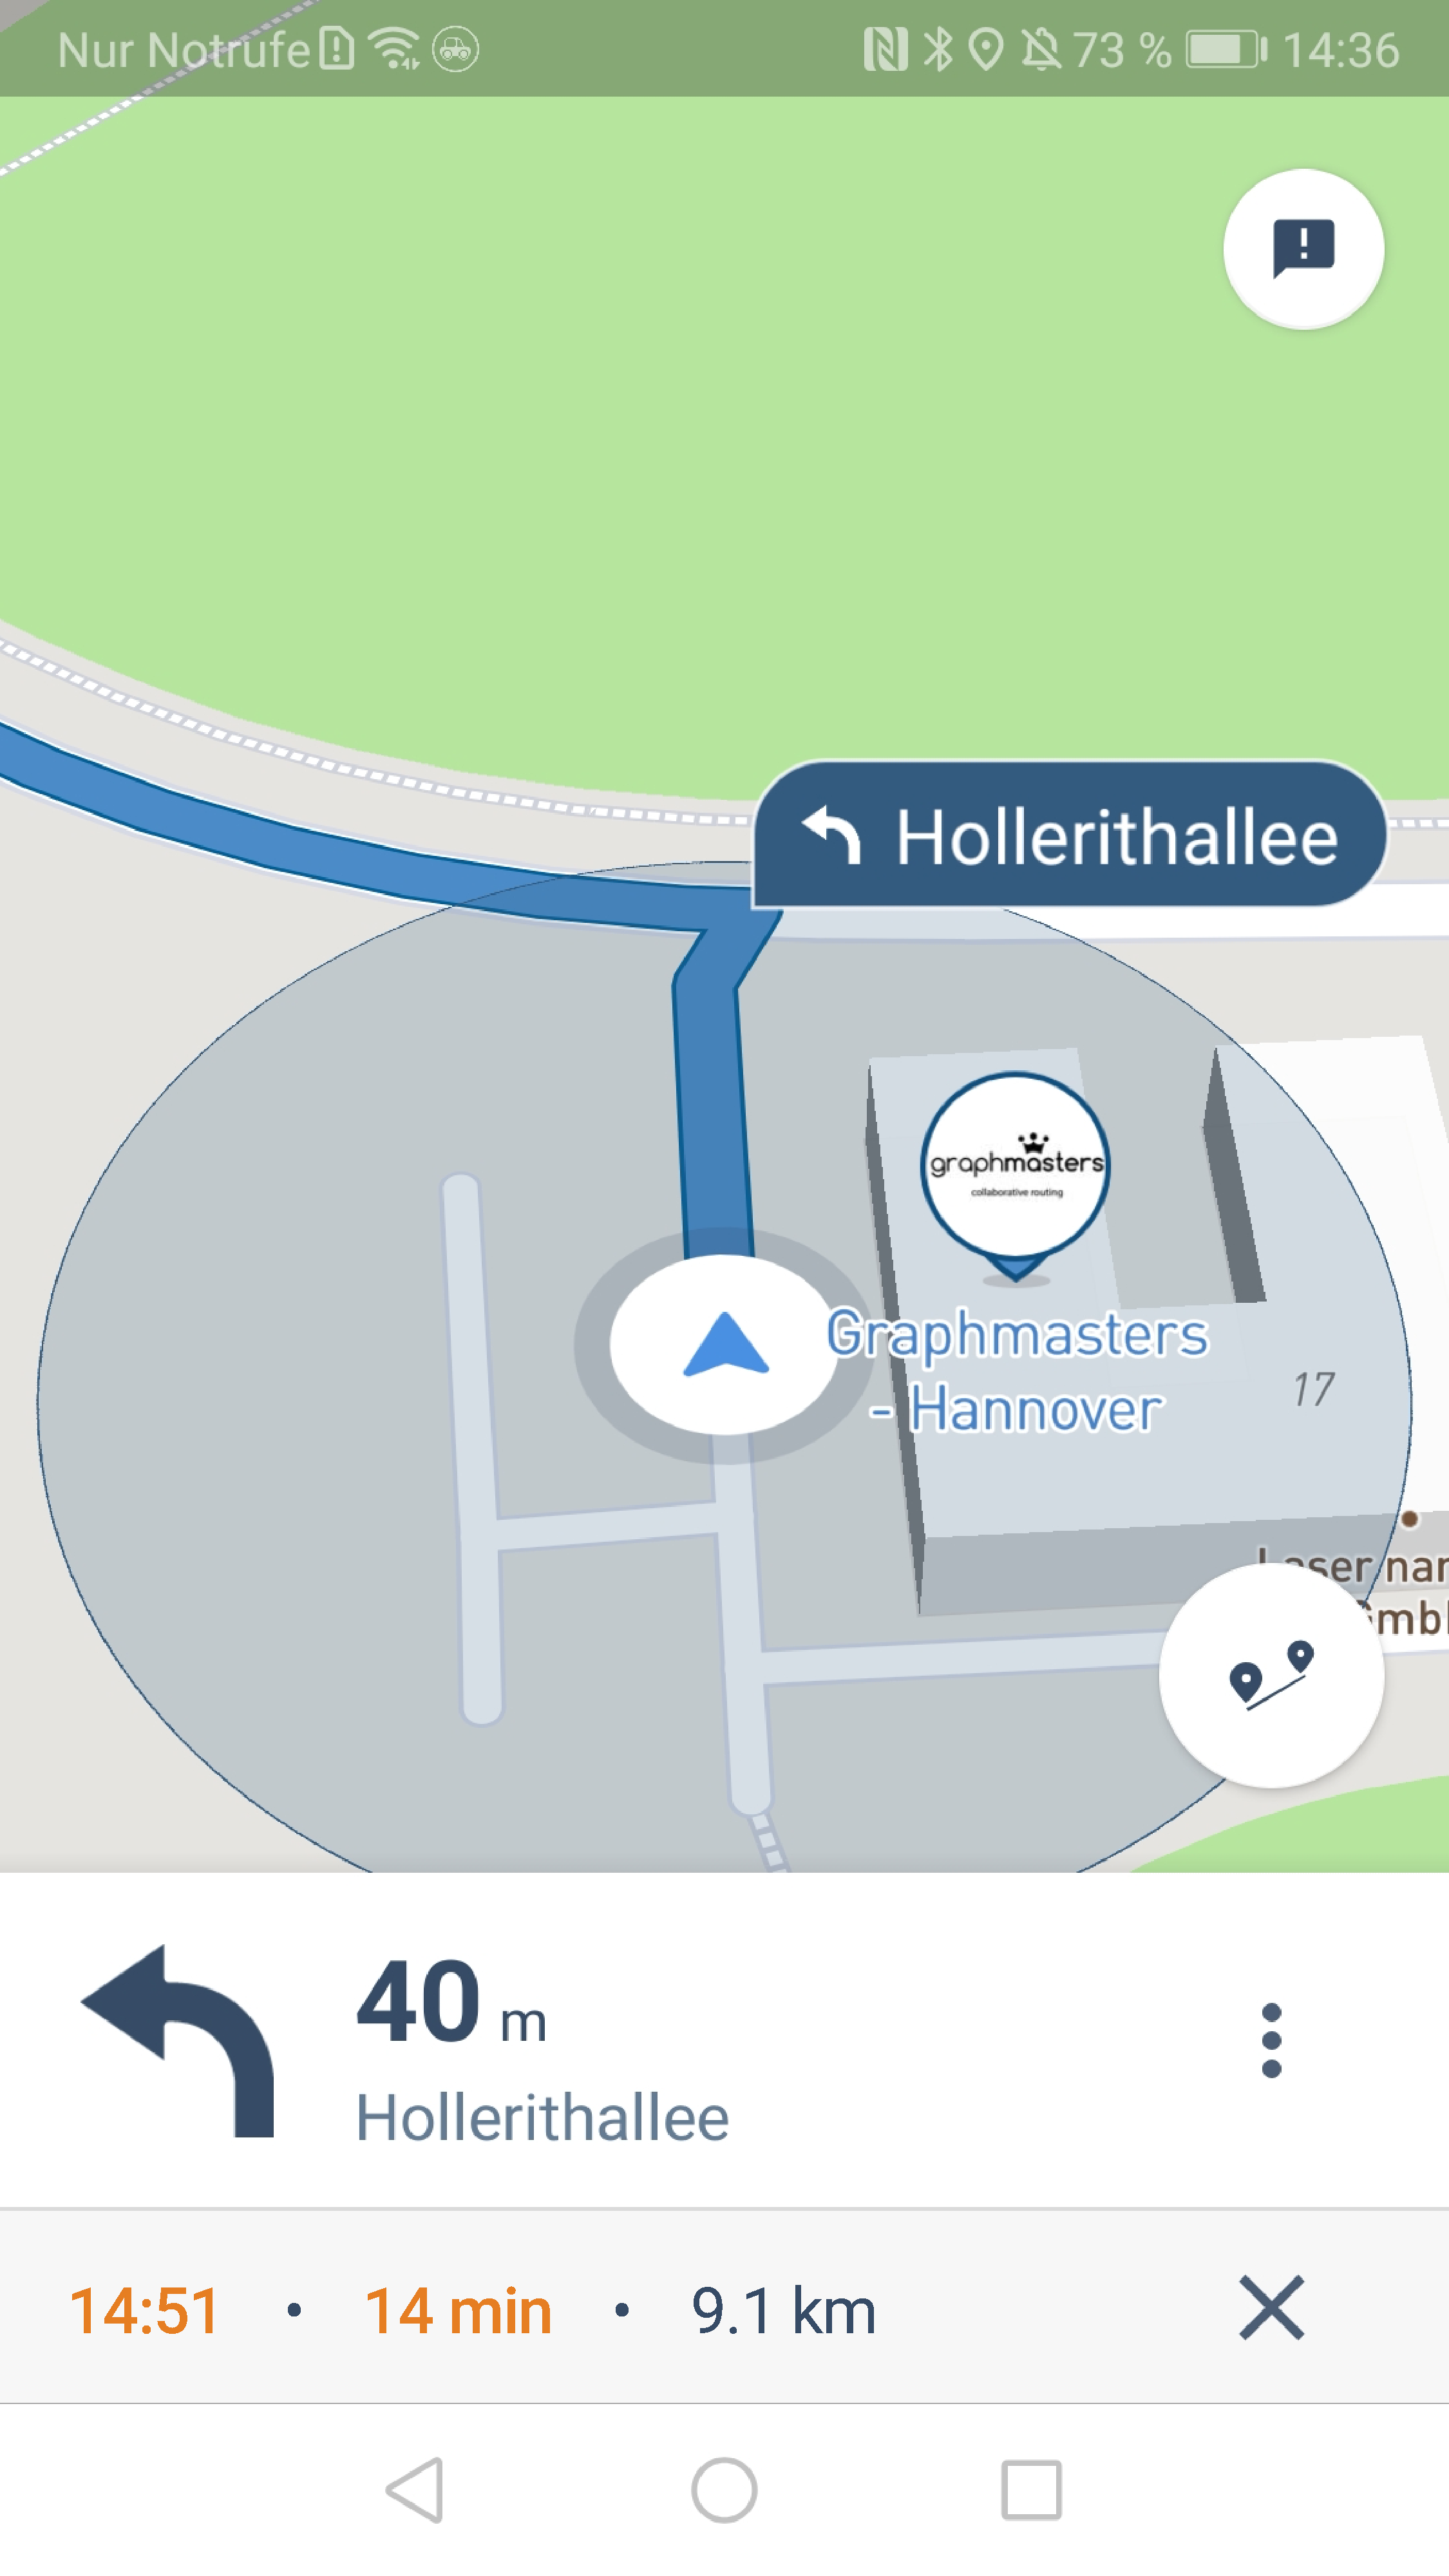
\includegraphics[width=.27\linewidth]{contents/06_model_evaluation/01_integration/res/03_traffic_volume/final_20.pdf}
    }
    \caption{Prototyp und finale Designs für die Erklärung zum kollaborativem Routing}
\end{figure}

\section{Themen der Reviews im Google Play Store und Apple App Store}
\label{sec:appendix_review_subjects}

\begin{table}[htb!]
    \begin{tabular}{p{.25\textwidth}p{.56\textwidth}p{.1\textwidth}}
        \hline
        Thema & Beschreibung        & Anzahl \\
        \toprule
        Feature Request             & Im Review werden neue Funktionen gefordert. & 18 \\
        \tablerowspacing
        Kollaboratives Routing      & Das Review deutet auf ein fehlendes Verständnis, was der Grundgedanke des
                                        kollaborativen Routings ist, hin. & 16 \\
        \tablerowspacing
        Schlechte Route             & Das Review enthält eine Beschwerde über eine bestimmte Routenführung. & 9 \\
        \tablerowspacing
        GPS-Verständnis             & Das Review deutet auf ein fehlendes Verständnis für schlechten GPS-Empfang hin. & 3 \\
        \tablerowspacing
        Offline-Modus-Verständnis   & Das Review deutet auf ein fehlendes Verständnis der Offline-Karten-Funktion 
                                        hin. & 3 \\
        \tablerowspacing
        Fehlende Information        & Das Review enthält eine Forderung nach mehr Informationen,
                                        die in NUNAV angezeigt werden sollen. & 3 \\
        \tablerowspacing
        Schlechte Suchergebnisse    & Im Review wird die Qualität der Suchergebnisse bemängelt. & 3 \\
        \tablerowspacing
        Verständnis Routenfarbe     & Im Review werden Nachfragen zur Einfärbung der Route gestellt. & 2 \\
        \tablerowspacing
        Falsche Kartendaten         & Im Review werden falsche Kartendaten bemängelt. & 1 \\
        \toprule
    \end{tabular}
\caption{Anzahl der Reviews im Google Play Store und Apple App Store mit mehrfach vorkommenden Themen}
\end{table}